\section{Modelowanie terenu (Bogna Lew)}
Do utworzenia terenu do gry wykorzystaliśmy zasób 3D World Building udostępniany przez Unity. Umożliwia on automatyczne
generowanie terenu na podstawie heightmapy - monochromatycznego obrazu reprezentującego model wysokościowy. Kolor czarny
reprezentuje najniższe punkty, natomiast kolor biały -  najwyższe.

\begin{figure}[h!]
    \centering
    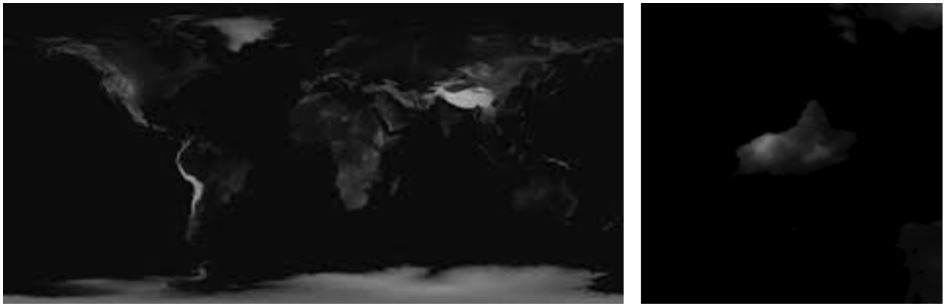
\includegraphics[width=0.9\textwidth]{images/modelowanie_terenu/przykladowe_heightmapy.jpg}
    \caption{Przykładowe heightmapy}\label{fig:przykladowe_heightmapy}
\end{figure}

Wygenerowanie terenu umożliwia narzędzie Terrain Toolbox, które można uruchomić wybierając z menu Window -> Terrain ->
Terrain Toolbox. Pozwala ono na ustawienie podstawowych parametrów takich jak długość, szerokość oraz wysokość terenu.
Należy również zaznaczyć checkbox Import Heightmap oraz załączyć obraz z modelem wysokościowym. Na koniec trzeba nacisnąć
przycisk Create, co spowoduje dodanie do sceny wygenerowanego terenu.

\begin{figure}[h!]
    \centering
    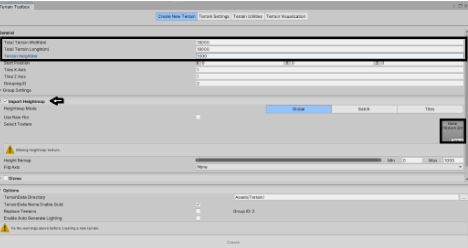
\includegraphics[width=0.6\textwidth]{images/modelowanie_terenu/generowanie.jpg}
    \caption{Widok na panel narzędzia Terrain Toolbox z zaznaczonymi wymienionymi sekcjami.}\label{fig:generowanie_terenu}
\end{figure}

Tak utworzony teren, chociaż już jest grywalny, posiada ostre i postrzępione krawędzie, które nie wyglądają zbyt
estetycznie. Wygładzenie ich poprawi wygląd terenu i sprawi, że będzie on bardziej realistyczny. Do tego służy narzędzie
Smooth Height dostępne w inspektorze terenu. Powoduje ono uśrednienie pobliskich płaszczyzn, co pozwala na usunięcie
nagłych zmian terenu i w rezultacie wygładzenie go.

\begin{figure}[h!]
    \centering
    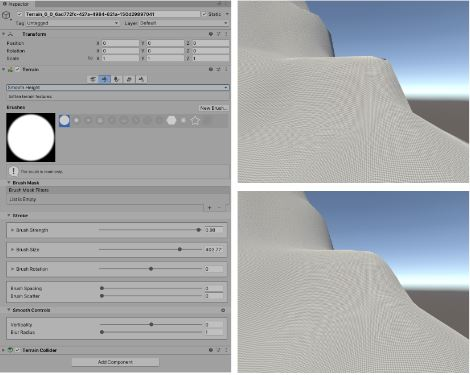
\includegraphics[width=0.8\textwidth]{images/modelowanie_terenu/rzezbienie.jpg}
    \caption{Widok panelu inspektora oraz terenu przed (górny) i po (dolny) zastosowaniu narzędzia Smooth Terrain.}\label{fig:rzezbienie_terenu}
\end{figure}

Kolejnym krokiem jest nałożenie tekstur. Służy do tego narzędzie Paint Texture. Umożliwia ono dodanie warstw, którymi
będzie można pokolorować teren. Warstwa znajdująca się najwyżej jest uznawana za domyślną i jej tekstura zostanie
nałożona na cały teren. Pozostałe warstwy natomiast stanowią swego rodzaju paletę kolorów, którymi można pomalować teren
za pomocą pędzla, który można wybrać w zakładce Brushes. W zakładce Stroke można ustawić podstawowe parametry pędzla
takie jak Brush Size oraz Brush Strength. Pierwszy parametr odnosi się do rozmiaru pędzla, a co za tym idzie obszaru na
który dana tekstura zostanie nałożona, natomiast drugi pozwala na określenie w jakim stopniu nakładany materiał zakryje
już nałożony.

\begin{figure}[h!]
    \centering
    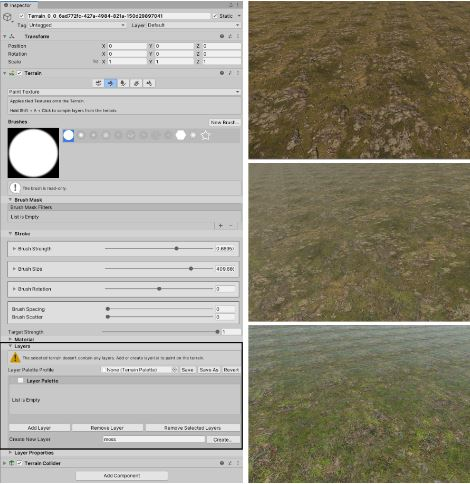
\includegraphics[width=0.8\textwidth]{images/modelowanie_terenu/tekstury.jpg}
    \caption{Widok panelu inspektora z wybranym narzędziem Paint Texture oraz efektu przed nałożeniem 2 tekstury (górny
    zrzut), po nałożeniu tekstury gdy Brush Strength wynosi 0.26 (środkowe zdjęcie) oraz gdy wynosi 0.67 (dolne).}\label{fig:malowanie_tekstur}
\end{figure}

Kolejną opcją udostępnianą przez Unity jest możliwość automatycznego ustawienia obiektów na mapie w losowy sposób,
dzięki narzędziu Paint Trees. Do udostępnianych przez nie parametrów należą między innymi Brush Size, działający
analogicznie jak poprzednio, oraz Tree Density, które definiuje średnią liczbę drzew umieszczanych na zdefiniowany
obszar. Obok przedstawiono przykładowy rezultat. Wykorzystano do tego paczkę LowPoly Trees and Rocks dostępną w Unity
Assets Store.

\begin{figure}[h!]
    \centering
    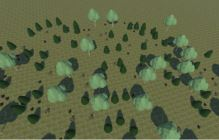
\includegraphics[width=0.5\textwidth]{images/modelowanie_terenu/drzewa.jpg}
    \caption{Widok na teren z drzewami.}\label{fig:pomalowane_drzewa}
\end{figure}

\begin{figure}[h!]
    \centering
    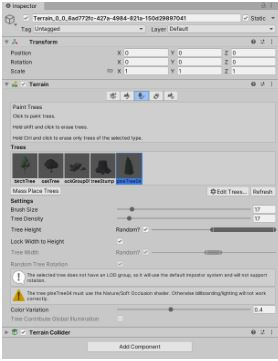
\includegraphics[width=0.6\textwidth]{images/modelowanie_terenu/malowanie_drzew.jpg}
    \caption{Widok na inspektor z włączonym narzędziem Paint Trees.}\label{fig:malowanie_drzew}
\end{figure}


